\section{Methodology}

%%%%%%%%%%%%%%%%%%%%%%%%%%%%%%%%%%%%%%%%%%%%%%%%%%%%%%%%%%%%%
% Mean Flow
%%%%%%%%%%%%%%%%%%%%%%%%%%%%%%%%%%%%%%%%%%%%%%%%%%%%%%%%%%%%%
\subsection{Mean Flow}

\begin{figure}[b]
  \centering
  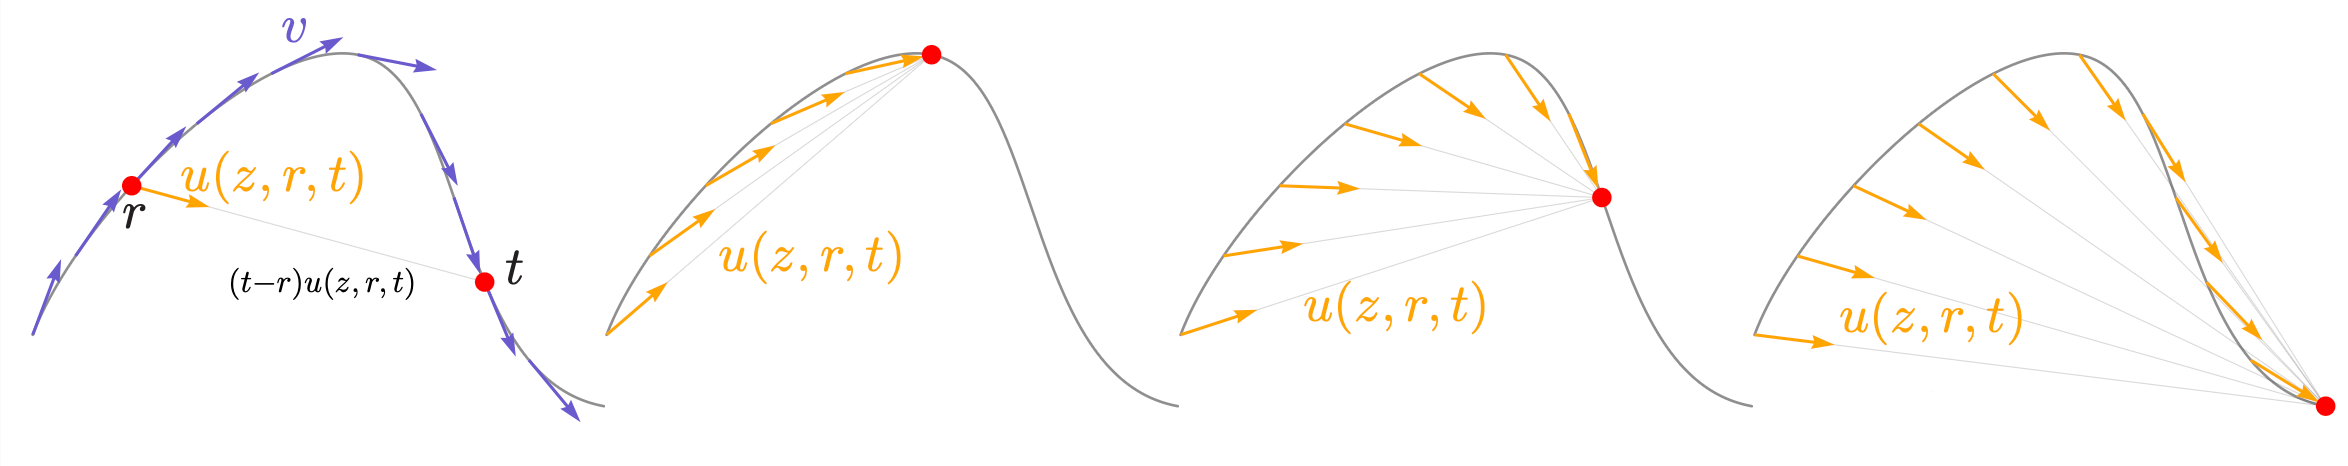
\includegraphics[width=\textwidth]{figures/meanflows.png}
  \caption{Illustration of the average velocity $u(z, r, t)$. Here, $z$ means the current location, i.e. $x_t$ in Equation~\eqref{average_velocity}. Leftmost: The instantaneous velocity $v(x_t, t)$. Right three subplots: The average velocity field at different time $t$. Figure revised from~\cite{meanflow}.}
  \vspace{-3em}
\end{figure}

Following~\cite{meanflow}, the instantaneous velocity field in Flow Matching can be replaced with an average velocity to enable one-step generation. Specifically, from time $r$ to time $t$, the average velocity is defined as:
%
\begin{equation}\label{average_velocity}
  u(x_t, r, t) \triangleq \frac{1}{t - r} \int^t_r v(x_\tau, \tau) \; d \tau.
\end{equation}
%
Rewrite Equation~\eqref{average_velocity} as $(t - r) u(x_t, r, t) = \int_r^t v(x_\tau, \tau) \, d \tau$, and differentiate both sides with respect to $t$:
%:
\begin{equation*}
  u(x_t, r, t) = v(x_t, t) - (t - r) \frac{d}{d t} u(x_t, r, t),
\end{equation*}
%
Applying the total derivative theorem, we obtain:
\begin{align}
  u(x_t, r, t) &= v(x_t, t) - (t - r) \left( \frac{\partial u}{\partial x_t} \frac{d x_t}{d t} + \frac{\partial u}{\partial r} \frac{d r}{d t} +  \frac{\partial u}{\partial t} \frac{d t}{d t} \right) \nonumber \\
  &= v(x_t, t) - (t - r) \left( \frac{\partial u}{\partial x_t} v(x_t, t) + \frac{\partial u}{\partial t}\right)
\end{align}
%
since $dr/dt = 0$ and $dx_t/dt = v(x_t, t)$.

Similiar to Flow Matching, we train a neural network $u^\theta(x_t, r, t)$ to approximate $u(x_t, r, t)$ with an MSE loss:
\begin{equation}
  \mathcal{L_\text{MF}} (\theta) = \mathbb{E}_{t, r, x_t \sim p_t} \left[ \left\| u^\theta(x_t, r, t) - \text{sg} \left[u^\text{tgt} (x_t, r, t)\right] \right\|_2^2 \right],
\end{equation}
%
where $\text{sg}\left[ \cdot \right]$ denotes the stop gradient operator and $u^\text{tgt}(x_t, r, t)$ is given by:
\begin{equation}
  u^\text{tgt} (x_t, r, t) =  v^\text{tgt}(x_t, t) - (t - r) \left( \frac{\partial u^\theta}{\partial x_t} v^\text{tgt}(x_t, t) + \frac{\partial u^\theta}{\partial t}\right).
\end{equation}
%
Here, the derivatives of $u$ are approximated by those of $u^\theta$, following~\cite{meanflow}.

Since the error term $u^\theta(x_t, r, t) - \text{sg} \left[u^\text{tgt} (x_t, r, t) \right]$ is a linear function of $v^\text{tgt}(x_t, t)$, and according to the result in Appendix~\ref{app:linear_func}, this allows $v^\text{tgt}(x_t, t)$ to be substituted with the conditional velocity $v(x_t, t \mid z)$:
%
\begin{align}
   \mathcal{L_\text{CMF}} (\theta) &= \mathbb{E}_{t, r, z \sim p_\text{target}, x_t \sim p_t(\cdot \mid z)} \left[ \left\| u^\theta(x_t, r, t) - \text{sg} \left[u^\text{tgt}_\text{cond} (x_t, r, t) \right] \right\|_2^2 \right] \\
   u^\text{tgt}_\text{cond} &=  v(x_t, t \mid z) - (t - r) \left( \frac{\partial u^\theta}{\partial x_t} v(x_t, t \mid z) + \frac{\partial u^\theta}{\partial t} \right)
\end{align}

This formulation allows MeanFlow to be trained similar to Flow Matching, while directly targeting an average velocity field that facilitates the one-step generation. Here, the derivative $\dfrac{d u^\theta}{d t}$ is computed by the
